\chapter{Widget Tree}

\section{Summary}
Developers utilise the widget tree to design user interfaces; they place widgets within each other to create basic and complicated layouts. Because almost everything in the Flutter framework is a widget, the code might get difficult to read when they start layering them. Developers can divide widgets into their own widget class, resulting in a shorter widget tree, which improves code readability and administration. Developers may take advantage of Flutter's subtree rebuilding, which enhances efficiency, by refactoring using a widget class. The widget is initialised to a final variable when you refactor with a constant. The chapter delves into refactoring with a method rather than a constant in depth. By invoking the method name, refactoring with a method returns the widget.\\

\begin{figure}[h]
  \begin{center}
  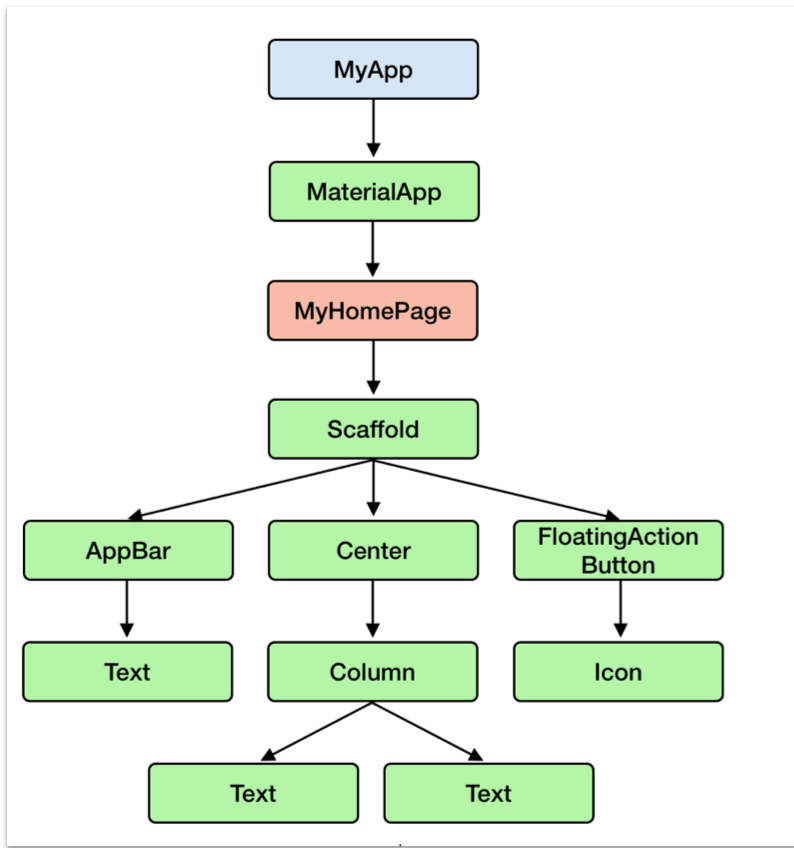
\includegraphics[height=120mm]{Images & Logos/CH_04_Widget_Tree.png}\\
  \end{center}
  \caption{Stateless Widget}
\end{figure}  
	